% !TeX document-id = {883512ec-ff7f-425c-a218-0c58e974f02f}
% !TeX root = stash.tex
% !TeX TXS-program:compile = txs:///pdflatex/[--shell-escape]
% !TeX encoding = UTF-8
% !TeX spellcheck = en_US
% https://orcid.org/0000-0003-4586-8500

% Other possible values are: 1610, 149, 54, 43 and 32.
% By default, it is to 128mm by 96mm(4:3)
\documentclass[aspectratio=169]{beamer}
%\setbeamertemplate{headline navigation symbols}{} 	% no navigation symbols
% \usetheme{Warsaw}
% \usecolortheme{seahorse}
% \usepackage[absolute,overlay]{textpos} % Text positioning

\usepackage{xcolor}

\title{Stash House}
\subtitle{A Toolkit to Collect and Hide Local Secrets}
\author{Franklin D.}
\institute{Recreational Computing Institute}
\date{2025}

\usepackage[T1]{fontenc}
\usepackage{lmodern}
\usepackage{tikz}
\usetikzlibrary{positioning,calc,shadings}

\tikzset{section number/.style={
		inner sep=0pt,
		draw=none,
	},
	section/.style={
		inner sep=0pt,
		draw=none,
		%text width=\the\dimexpr\paperwidth-3.8em\relax,
		text=blue,
		align=center
	},
	subsection/.style={
		inner sep=0pt,
		draw=none,
		%text width=\the\dimexpr\paperwidth-3.8em\relax,
		text=gray,
		align=center
	}
}

\makeatletter
\def\sectionsubtitle#1{\gdef\@sectionsubtitle{#1}}
\AtBeginSection[]{
	\begingroup
	% Lighter, beamer native version
	\setbeamercolor{background canvas}{bg=gray!30}
	%
	\begin{frame}
		\begin{tikzpicture}[remember picture,overlay]
			\coordinate[yshift=-10mm] (rectsouthwest) at (current page.north west);
			\coordinate[yshift=-10mm] (rectsoutheast) at (current page.north east);
			\fill[white] (current page.north west) rectangle (rectsoutheast);
			\shade [left color=gray,right color=white] (rectsouthwest) rectangle +(\paperwidth,-0.02);
			\node[section,anchor=center] at (current page.center) (title) {\fontsize{20}{20}\selectfont\insertsectionhead};
			\node[subsection,below=5mm of title]  (subtitle) {\@sectionsubtitle};
		\end{tikzpicture}
	\end{frame}
	\gdef\@sectionsubtitle{}
	\endgroup
}
\makeatother

%%%%%%%%%%%%%%%%%%%%%%%%%%%%%%%%%%%%%%%%%  Notes pages

% These slides also contain speaker notes. You can print just the slides,
% just the notes, or both, depending on the setting below. Comment out the want
% you want.

%\setbeameroption{hide notes} % Only slides
%\setbeameroption{show only notes} % Only notes
%\setbeameroption{show notes on second screen=right} % Both

% To give a presentation with the Skim reader (http://skim-app.sourceforge.net) on OSX so
% that you see the notes on your laptop and the slides on the projector, do the following:
%
% 1. Generate just the presentation (hide notes) and save to slides.pdf
% 2. Generate onlt the notes (show only nodes) and save to notes.pdf
% 3. With Skim open both slides.pdf and notes.pdf
% 4. Click on slides.pdf to bring it to front.
% 5. In Skim, under "View -> Presentation Option -> Synhcronized Noted Document"
%    select notes.pdf.
% 6. Now as you move around in slides.pdf the notes.pdf file will follow you.
% 7. Arrange windows so that notes.pdf is in full screen mode on your laptop
%    and slides.pdf is in presentation mode on the projector.

% Give a slight yellow tint to the notes page
%\setbeamertemplate{note page}{\pagecolor{yellow!5}\insertnote}\usepackage{palatino}
%\setbeamertemplate{note page}{\pagecolor{yellow!5}\vfill\insertnote\vfill}

%\setbeamertemplate{note page}{%
%	\pagecolor{yellow!5}
%	\vfill
%	\begin{minipage}[c][\textheight][t]{\textwidth}
%		{\usebeamerfont{frametitle}\usebeamercolor[fg]{frametitle}\insertframetitle\par}
%		\insertnote
%	\end{minipage}
%}

% customize the caption on figures
\setbeamertemplate{caption}[numbered]
\setbeamerfont{caption}{size=\large}
\setbeamercolor{caption}{fg=white}
\setbeamercolor{caption name}{fg=white}

\begin{document}

{
\usebackgroundtemplate{
\includegraphics[width=\paperwidth]{../static/images/technology-presentation.jpg}}%
\begin{frame}
	% \titlepagestash apply
    \note[item]{https://www.youtube.com/watch?v=DYDT165LGBY}
\end{frame}
}

%\begin{frame}
%	\frametitle{Table of Contents}
%	\tableofcontents
%\end{frame}



% you can uncomment one of these for the whole doc, or add at the start of each section as desired
\usebackgroundtemplate{
\includegraphics[width=\paperwidth]{../static/images/section.jpg}}
%\usebackgroundtemplate{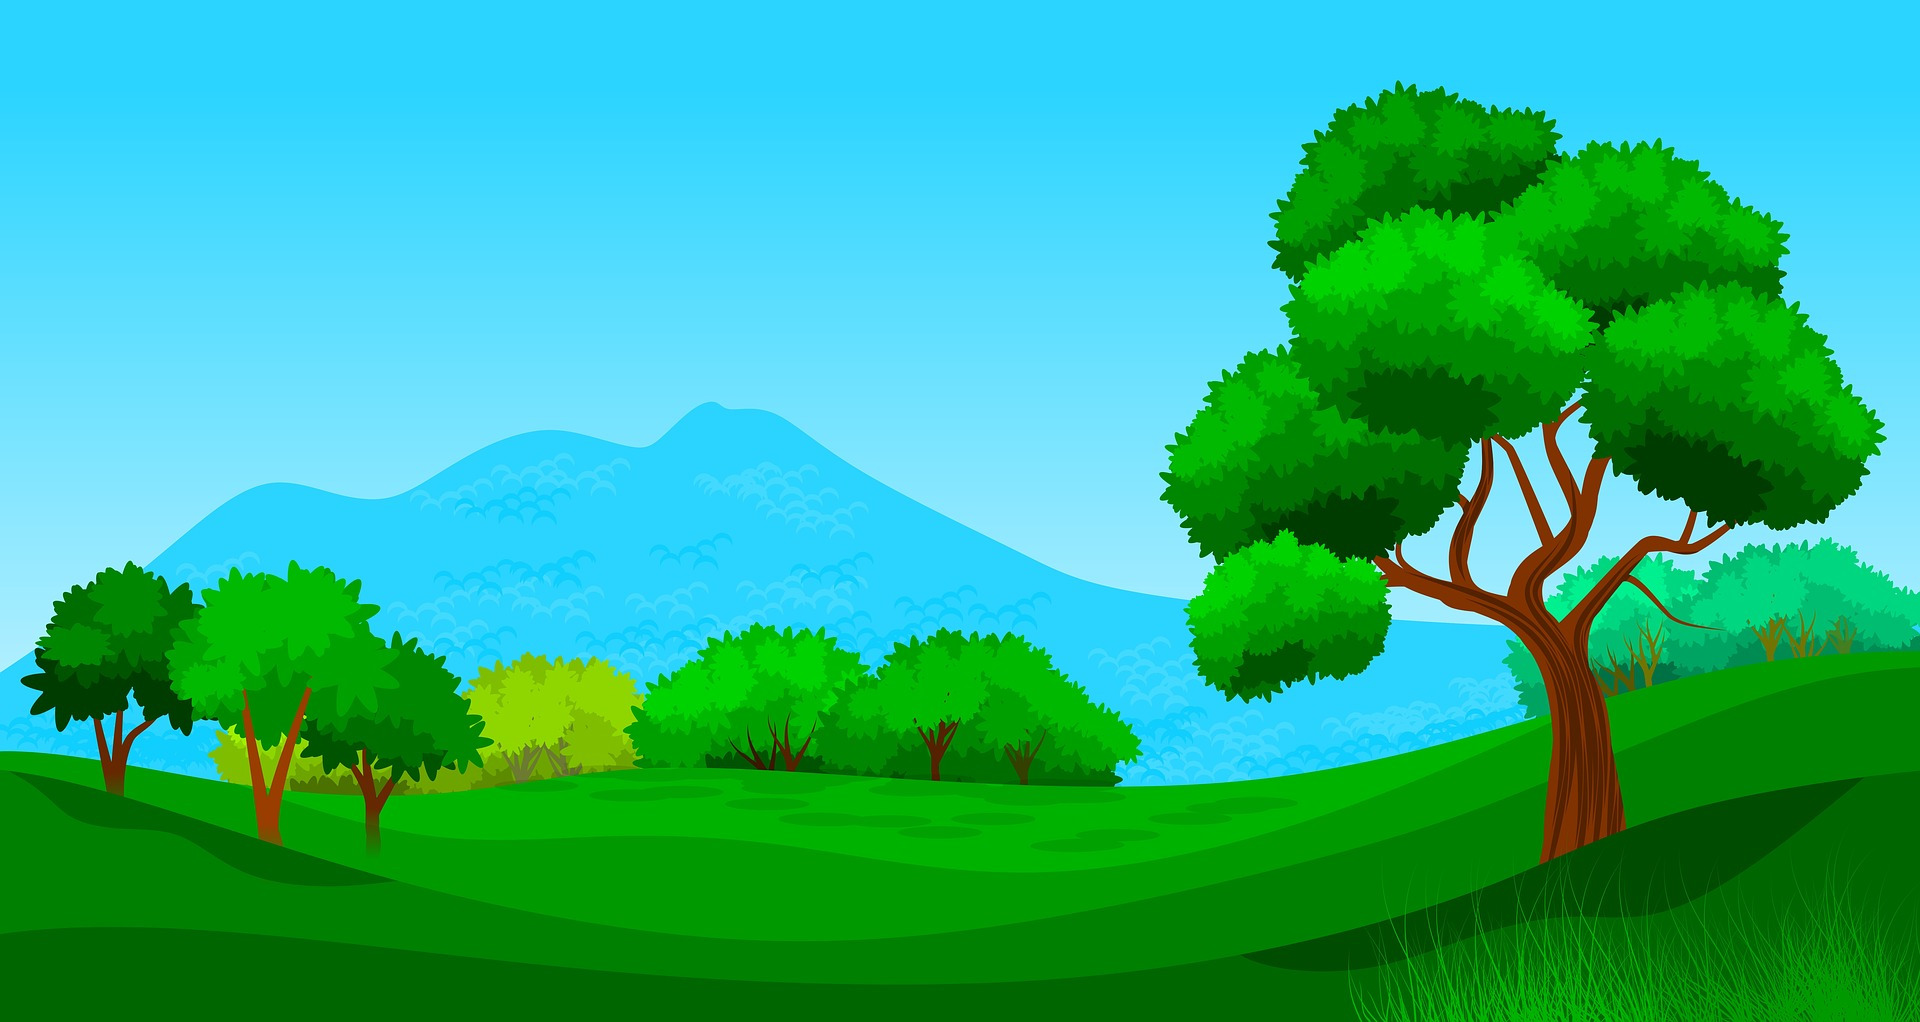
\includegraphics[width=\paperwidth]{../images/landscape.jpg}}
%\usebackgroundtemplate{
\includegraphics[width=\paperwidth]{../images/tree.jpg}}
\sectionsubtitle{\textcolor{black}{The Lost Art of Keeping a Secret}}
\section{Introduction}

{
	\usebackgroundtemplate{
\includegraphics[width=\paperwidth]{../static/images/tech-white.jpg}}%
	\begin{frame}
	\frametitle{Step One: Admit That You Have a Problem}
	\begin{columns}
		\column{0.5\textwidth}
		Most of us have a (reasonable?) expectation of trust for the files on our local machine. And so, we leave things like saved passwords and other credentials and secrets pasted into text files for quick access.
		\column{0.5\textwidth}
		\begin{figure}
            \centering
            
\includegraphics[width=0.77\textwidth]{../static/images/problem.jpg}
            \caption{You}
            \label{fig:question}
        \end{figure}

    \end{columns}
    \note[item]{Yes you do this}
\note[item]{No it's not good}


\end{frame}
}

{
	\usebackgroundtemplate{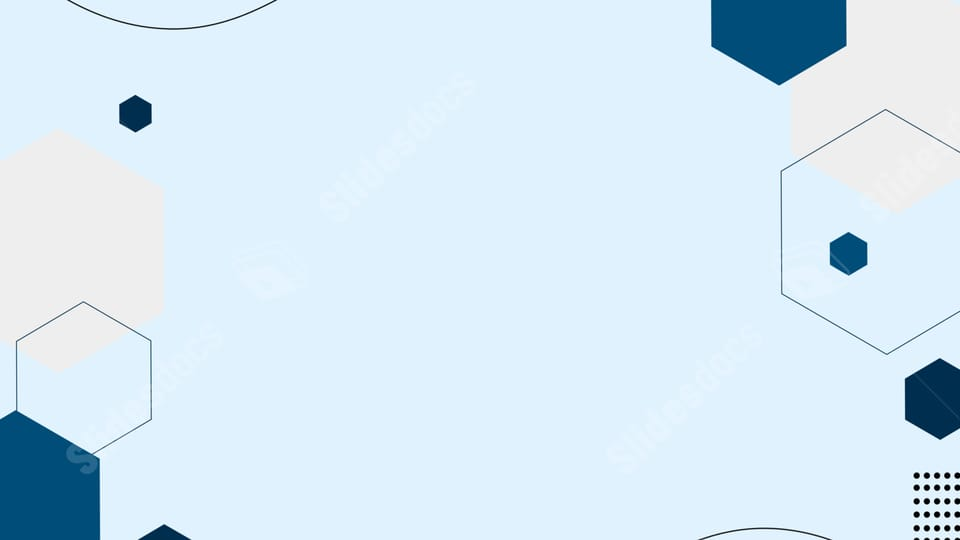
\includegraphics[width=\paperwidth]{../static/images/tech-back.jpg}}%
	\begin{frame}
		\frametitle{\textcolor{black}{Requisite Bio Slide}}
		\begin{itemize}
			\item {I have been doing things to computers for a long time.}
			\item {During the day I am a computer security consultant at a big company.}
			\item {I teach in the afternoons.}
			\item {\href{https://g.dev/franklin}{Some of my background is at this link https://g.dev/franklin}}
		\end{itemize}
		\note[item]{link to socials or something}
	\end{frame}
}

\usebackgroundtemplate{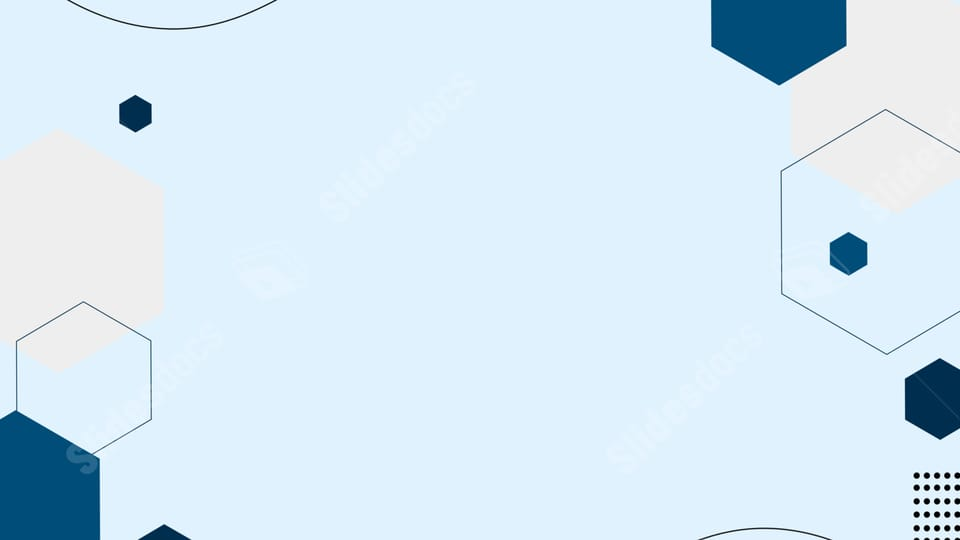
\includegraphics[width=\paperwidth]{../static/images/tech-back.jpg}}
\begin{frame}
    \frametitle{Project Goals}
    \begin{itemize}
        \item Locate unprotected credentials on the local host
        \item Encrypt and safely store these credentials and other secrets.
        \item Access to credential store from multiple locations.
        \item We gain the ability to use our encrypted secrets in our applications.
    \end{itemize}

    \note[item]{Clean up the ones we know about}
    \note[item]{Of course there will always be gaps and edge cases, just try to improve over time}
    \note[item]{What prior art is out there}

\end{frame}


\begin{frame}
    \frametitle{Setting Up your Haunted Stash House}
    These are the basic setup steps so you have a place to hide your secrets.
    \begin{itemize}
        \item Create a repository on GitHub or other revision control system.
        \item Install the framework (demo soon).
        \item Set up your GPG key.
        \item Add items to DB, remove plain text tokens and secrets.
    \end{itemize}
    In the following slides we will break each of these items down.
\end{frame}

\begin{frame}
    \frametitle{Demo Script: Setup}
    \begin{itemize}
        \item \href{ https://github.com/devsecfranklin/stash-house/blob/main/bin/install-client.sh }{Here is a stash-house setup tool that you can use/modify for your system. }    \note[item]{Yes you do this}
        \note[item]{No it's not good}
        
        \item ``https://github.com/devsecfranklin/stash-house''
    \end{itemize}
    \note[item]{Do a small demo here}
    \note[item]{May want to have a video ready just in case}
\end{frame}


{
\usebackgroundtemplate{
\includegraphics[width=\paperwidth]{../static/images/section.jpg}}
\sectionsubtitle{\textcolor{black}{What is it you want to protect?}}
\section{Finding and Protecting Secrets}
}

{
	\usebackgroundtemplate{
\includegraphics[width=\paperwidth]{../static/images/tech-white.jpg}}%%
\begin{frame}
	\frametitle{What Do We Mean by Secrets, Exactly}
	\begin{itemize}
		\item Credentials for example a username/password for that lab host that you only need for a couple weeks.
		\item Text files that are used as keys.
	\end{itemize}

    \note[item]{In my case I had a whole folder of text files that I'd collected of some time.}

\end{frame}
}

{
	\usebackgroundtemplate{
\includegraphics[width=\paperwidth]{../static/images/tech-white.jpg}}%
\begin{frame}
	\frametitle{The Process of Finding Secrets}
	\begin{itemize}
		\item Look around your local machines for tokens and credentials.
		\item Use some automation to help you find them.
	\end{itemize}
	\note[item]{There are some known places we can look}
	\note[item]{Clean up the ones we know about}
\end{frame}
}

\usebackgroundtemplate{
\includegraphics[width=\paperwidth]{../static/images/tech-white.jpg}}%
\begin{frame}
	\frametitle{Demo Script: Scanning Your Local System}
	\begin{itemize}
        \item\href{ https://github.com/devsecfranklin/stash-house/tree/main/demo/01_scanner}{Here is a small tool that you can use/modify for your system}
	\end{itemize}
	\note[item]{Do a small demo here}
\end{frame}

{
	\usebackgroundtemplate{
\includegraphics[width=\paperwidth]{../static/images/section.jpg}}
	\sectionsubtitle{We found the secrets, now what?}
	\section{Hide Your Goodies}
}


\begin{frame}
    \frametitle{Setting up GnuPG}
	\begin{itemize}
	\item \href{https://docs.github.com/en/authentication/managing-commit-signature-verification/generating-a-new-gpg-key}{GPG key setup.}
	\item 
\end{itemize}
\note[item]{\href{https://devhints.io/gnupg}{There is a cheat sheet here.}}
\end{frame}

\begin{frame}
	\frametitle{Storing Tokens at Rest}
    We will use a tool called pass in combination with out GnuPG key to encrypt the secrets we found.
	\begin{itemize}
        \item Okay we found some, now what?
		\item Encrypt the tokens and push them into a Revision Control System.
        \item Could be a ``private repo'' but it doesn't have to.
	\end{itemize}
\end{frame}

\begin{frame}
	\frametitle{Saving Simple Tokens}
	\begin{itemize}
		\item Use the pass tool to encrypt the tokens and push them into Revision Control.
	\end{itemize}
    \note[item]{test}
\end{frame}

\begin{frame}
	\frametitle{Saving Multi-line Tokens}
	\begin{itemize}
		\item Use pass to encrypt a multi-line secret and push it into Revision Control.
	\end{itemize}
    \note[item]{We can also save multi-line secrets, GCloud JSON for example.}
\end{frame}

\begin{frame}
	\frametitle{Backing up Tokens to RCS}
	\begin{itemize}
		\item Encrypt the tokens and secrets
		\item Push everything into revision control.
	\end{itemize}
\end{frame}

{
\usebackgroundtemplate{
\includegraphics[width=\paperwidth]{../static/images/section.jpg}}
\sectionsubtitle{\textcolor{black}{How to Use What You Built}}
\section{Using Your Stashed Tokens}
}

\usebackgroundtemplate{
\includegraphics[width=\paperwidth]{../static/images/tech-white.jpg}}%
\begin{frame}
	\frametitle{Using Tokens}
	\begin{itemize}
		\item Now you can use the secrets in your project without exposing them.
	\end{itemize}
\end{frame}

\begin{frame}
	\frametitle{Considerations}
	\begin{itemize}
		\item You need your GPG key on the local machine to encrypt, decrypt, and use the secrets.
	\end{itemize}
\note[item]{Don't be lazy, you still have to use a password manager}
\end{frame}

{
\usebackgroundtemplate{
\includegraphics[width=\paperwidth]{../static/images/section.jpg}}
\sectionsubtitle{\textcolor{black}{Where is all this going?}}
\section{Other Cool Stuff}
}

\begin{frame}
    \frametitle{Keyringer}
    \begin{itemize}
        \item I found a tool called ``keyringer'' that is supposed to do all this already.
        \item ``Keyringer lets you manage and share secrets using GnuPG and Git in a distributed fashion.''
        \item I will incorporate it into this tool set if that makes sense.
    \end{itemize}
    \note[item]{It has custom commands to encrypt, decrypt and re-crypt secrets as well as create key pairs and supports encryption to multiple recipients and groups of different recipients to ensure the same repository can be shared with a work group but allowing to keep some secrets available just to subsets of that group.
    	
    OpenSSL is needed to generate X.509 certificates and keys and xdg-utils are needed to open and edit encrypted secrets according to their file types. }
\end{frame}

\begin{frame}
    \frametitle{Nostr}
    \begin{itemize}
        \item Been experimenting with the decentralized ideas from the coin mining world.
        \item There are all sorts of apps and clients out there.
    \end{itemize}
    \note[item]{Try and include an update before presentation}
\end{frame}

\begin{frame}
	\frametitle{Kerberos and OpenLDAP}
	\begin{itemize}
		\item Research if there is any possible overlap.
		\item Integration with Kerberos on a LAN?
	\end{itemize}
	\note[item]{Research if there is any possible overlap.}
\end{frame}

\begin{frame}
    \frametitle{demo container}
    \begin{itemize}
        \item There is a container file in the project repo.
    \end{itemize}
    \note[item]{Try and include this tool before presentation}
\end{frame}

\begin{frame}
	\frametitle{SSH Key Setup}
	\begin{itemize}
		\item 
	\end{itemize}
	\note[item]{We will use the same repository as this slide deck is stored in for demonstration purposes.}
	\note[item]{May want to have a video ready just in case}
\end{frame}

\begin{frame}
	\frametitle{Github Setup}
	\begin{itemize}
		\item 
	\end{itemize}
	\note[item]{We will use the same repository as this slide deck is stored in for demonstration purposes.}
	\note[item]{May want to have a video ready just in case}
\end{frame}

\end{document}
